Un moteur d'exécution, ou {\em runtime}, est un morceau de logiciel utilisé par d'autres logiciels pour abstraire des parties du système.
%
L'idée principale est {\em compiler une fois, exécuter partout}.
%
Ils sont présent un peu partout et peuvent avoir différentes fonctions.
%
Certains langages dits de haut niveau utilisent un runtime, par exemple Java a un runtime pour gérer son ramasse-miettes.
%
Toutes les implémentations de MPI ont un runtime.
%
Les cadriciels de programmation à base de tâches tendent à utiliser un runtime.
%
Les parties suivantes se concentreront sur le support des runtimes pour la programmation à base de tâches.


Les runtimes utilisés pour la programmation à base de tâches doivent en premier lieu être capable d'ordonnancer le traitement des tâches tout en respectant l'ordre des dépendances entre les tâches (Fig~\ref{fig:runtime}).
%
Ces runtime doivent aussi fournir un équilibrage de charge entre toutes les ressources matérielles disponibles (potentiellement hétérogènes) dans le but de minimiser le temps de calcul.
%
Certains runtimes s'occupent de transférer des données entre deux ressources potentiellement hétérogènes, comme par exemple entre la mémoire principale et la mémoire d'une carte graphique ou plus simplement entre deux processus.
%
Ces transferts peuvent être implicites, le runtime a connaissance des données qui sont manipulées, ou ils peuvent être explicites avec l'utilisation d'une tâche spéciale qui s'occupera de faire les échanges de données.

%   (-_-)   %
\begin{figure}[t!]
  \centering
  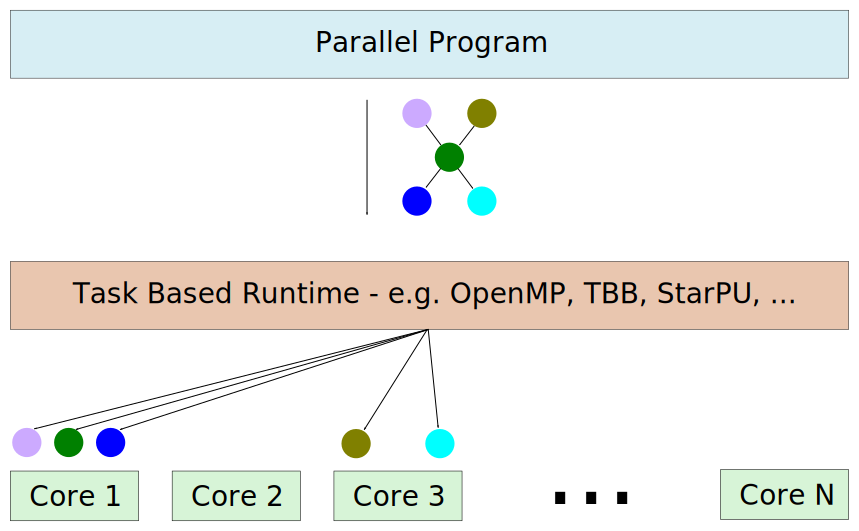
\includegraphics[width=0.8\textwidth]{runtime}
  \caption{Le programme parallèle fournit un graphe de tâches à l'ordonnanceur de tâches. Les tâches sont ensuite distribuées sur les coeurs de calcul disponibles.}
  \label{fig:runtime}
\end{figure}


Pour améliorer l'équilibrage de charge, les runtimes ont des politiques d'ordonnancement, la plupart de ces politiques sont dynamiques et peuvent s'adapter à la charge courante de la machine.
%
D'autres politiques d'ordonnancement, dîtes statiques, permettent de réduire le coût d'ordonnancement.
%
L'ordonnanceur parfait n'existe pas et n'existera sûrement jamais.
%
En effet, trouver le meilleur ordonnancement d'un ensemble de tâches avec un nombre limité de ressources de calcul est un problème NP-complet\footnote{Un problème est NP-complet si le temps nécessaire à la résolution du problèmes est polynomial comparé à la taille des données en entrées et que ce problème soit aussi difficile que tous les autres problèmes NP-complets.}.
%
Il existe des heuristiques d'ordonnancement qui donnent de bons résultats dans la majorité des cas, nous pouvons citer l'algorithme HEFT\cite{heft}.
%
Si le modèle de programmation le permet, des informations additionnelles peuvent être attribuées aux tâches, comme par exemple une estimation du temps de calcul, ces informations sont ensuite utilisées par l'ordonnanceur pour améliorer le placement des tâches.


L'apparition des premières machines parallèles à mémoire partagée a conduit à la recherche de nouvelles méthodes pour les programmer.
%
Il faut donc distribuer une charge de travail sur plusieurs unités de calcul.
%
Malheureusement, il arrive que cette charge de travail de soit pas connu l'avance.
%
Une idée est alors apparu pour rendre cette distribution plus flexible : le vol de travail (ou {\em work-stealing} en anglais).
%
Dès qu'une ressource de calcul n'as plus de travail, elle essaye de voler du travail à une autre ressource.
%
Le langage Cilk~\cite{Cilk}, apparu en 1994 et toujours développé sous le nom Cilk++~\cite{Cilk++}, permet de faire du vol de travail.
%
Les tâches sont décrites par le programmeur avec des mots clés additionnels au langage C, par exemple le mot-clé {\em spawn} placé avant l'appel d'une fonction permet à Cilk de comprendre qu'il doit créer une nouvelle tâche et qu'il doit l'ordonnancer.
%
Ces tâches sont empilées sur une pile spécifique à chaque thread.
%
Le vol de tâche se fait par le biais de cette pile de tâches.


Peu de temps après, en 1997, une interface de programmation parallèle voit le jour, il s'agit d'OpenMP~\cite{OpenMP}.
%
Les premières versions d'OpenMP se concentrent sur le parallélisme de boucle.
%
Ce n'est qu'en 2008 que le support des tâches est ajouté à OpenMP dans sa version 3.0.


Plus récemment, à la fin des années 2000, la révolution du GPGPU donne lieu à l'apparition de nouveaux runtime.
%
Ces runtimes gèrent désormais des ressources hétérogènes avec des espaces d'adressage mémoire différents.
%
Ils doivent donc prendre en charge la cohérence mémoire entre les espaces d'adressage.
%
Parmi ces runtimes on trouve StarPU~\cite{starpu}, PaRSEC~\cite{PaRSEC}, X-KAAPI~\cite{xkaapi} et OMPSs~\cite{OMPSs}.
%
Le parallélisme de boucle sur architectures hétérogène a aussi eu droit à une spécification, il s'agit d'OpenACC~\cite{OpenACC}.
